        \begin{concept}
            \vocab{Non-linear} behavior cannot be accurately represented by any \gren{linear} model. 
    
            In order to create an accurate model, we have to use some \purp{nonlinear} operation.
        \end{concept}
    
        If we could create effective, non-linear models, we might even be able to deal with data that was previously "\textbf{linearly inseparable}".

    \subsecdiv

    \subsection*{Possible Solutions: Polynomials}

        Let's try to think of ways to approach this problem. We'll start with a 1-D input, for simplicity.

        Upon hearing "non-linear", we might remember the function we introduced last chapter: the \textbf{sigmoid}.
    
        \begin{figure}[H]
            \centering
            
            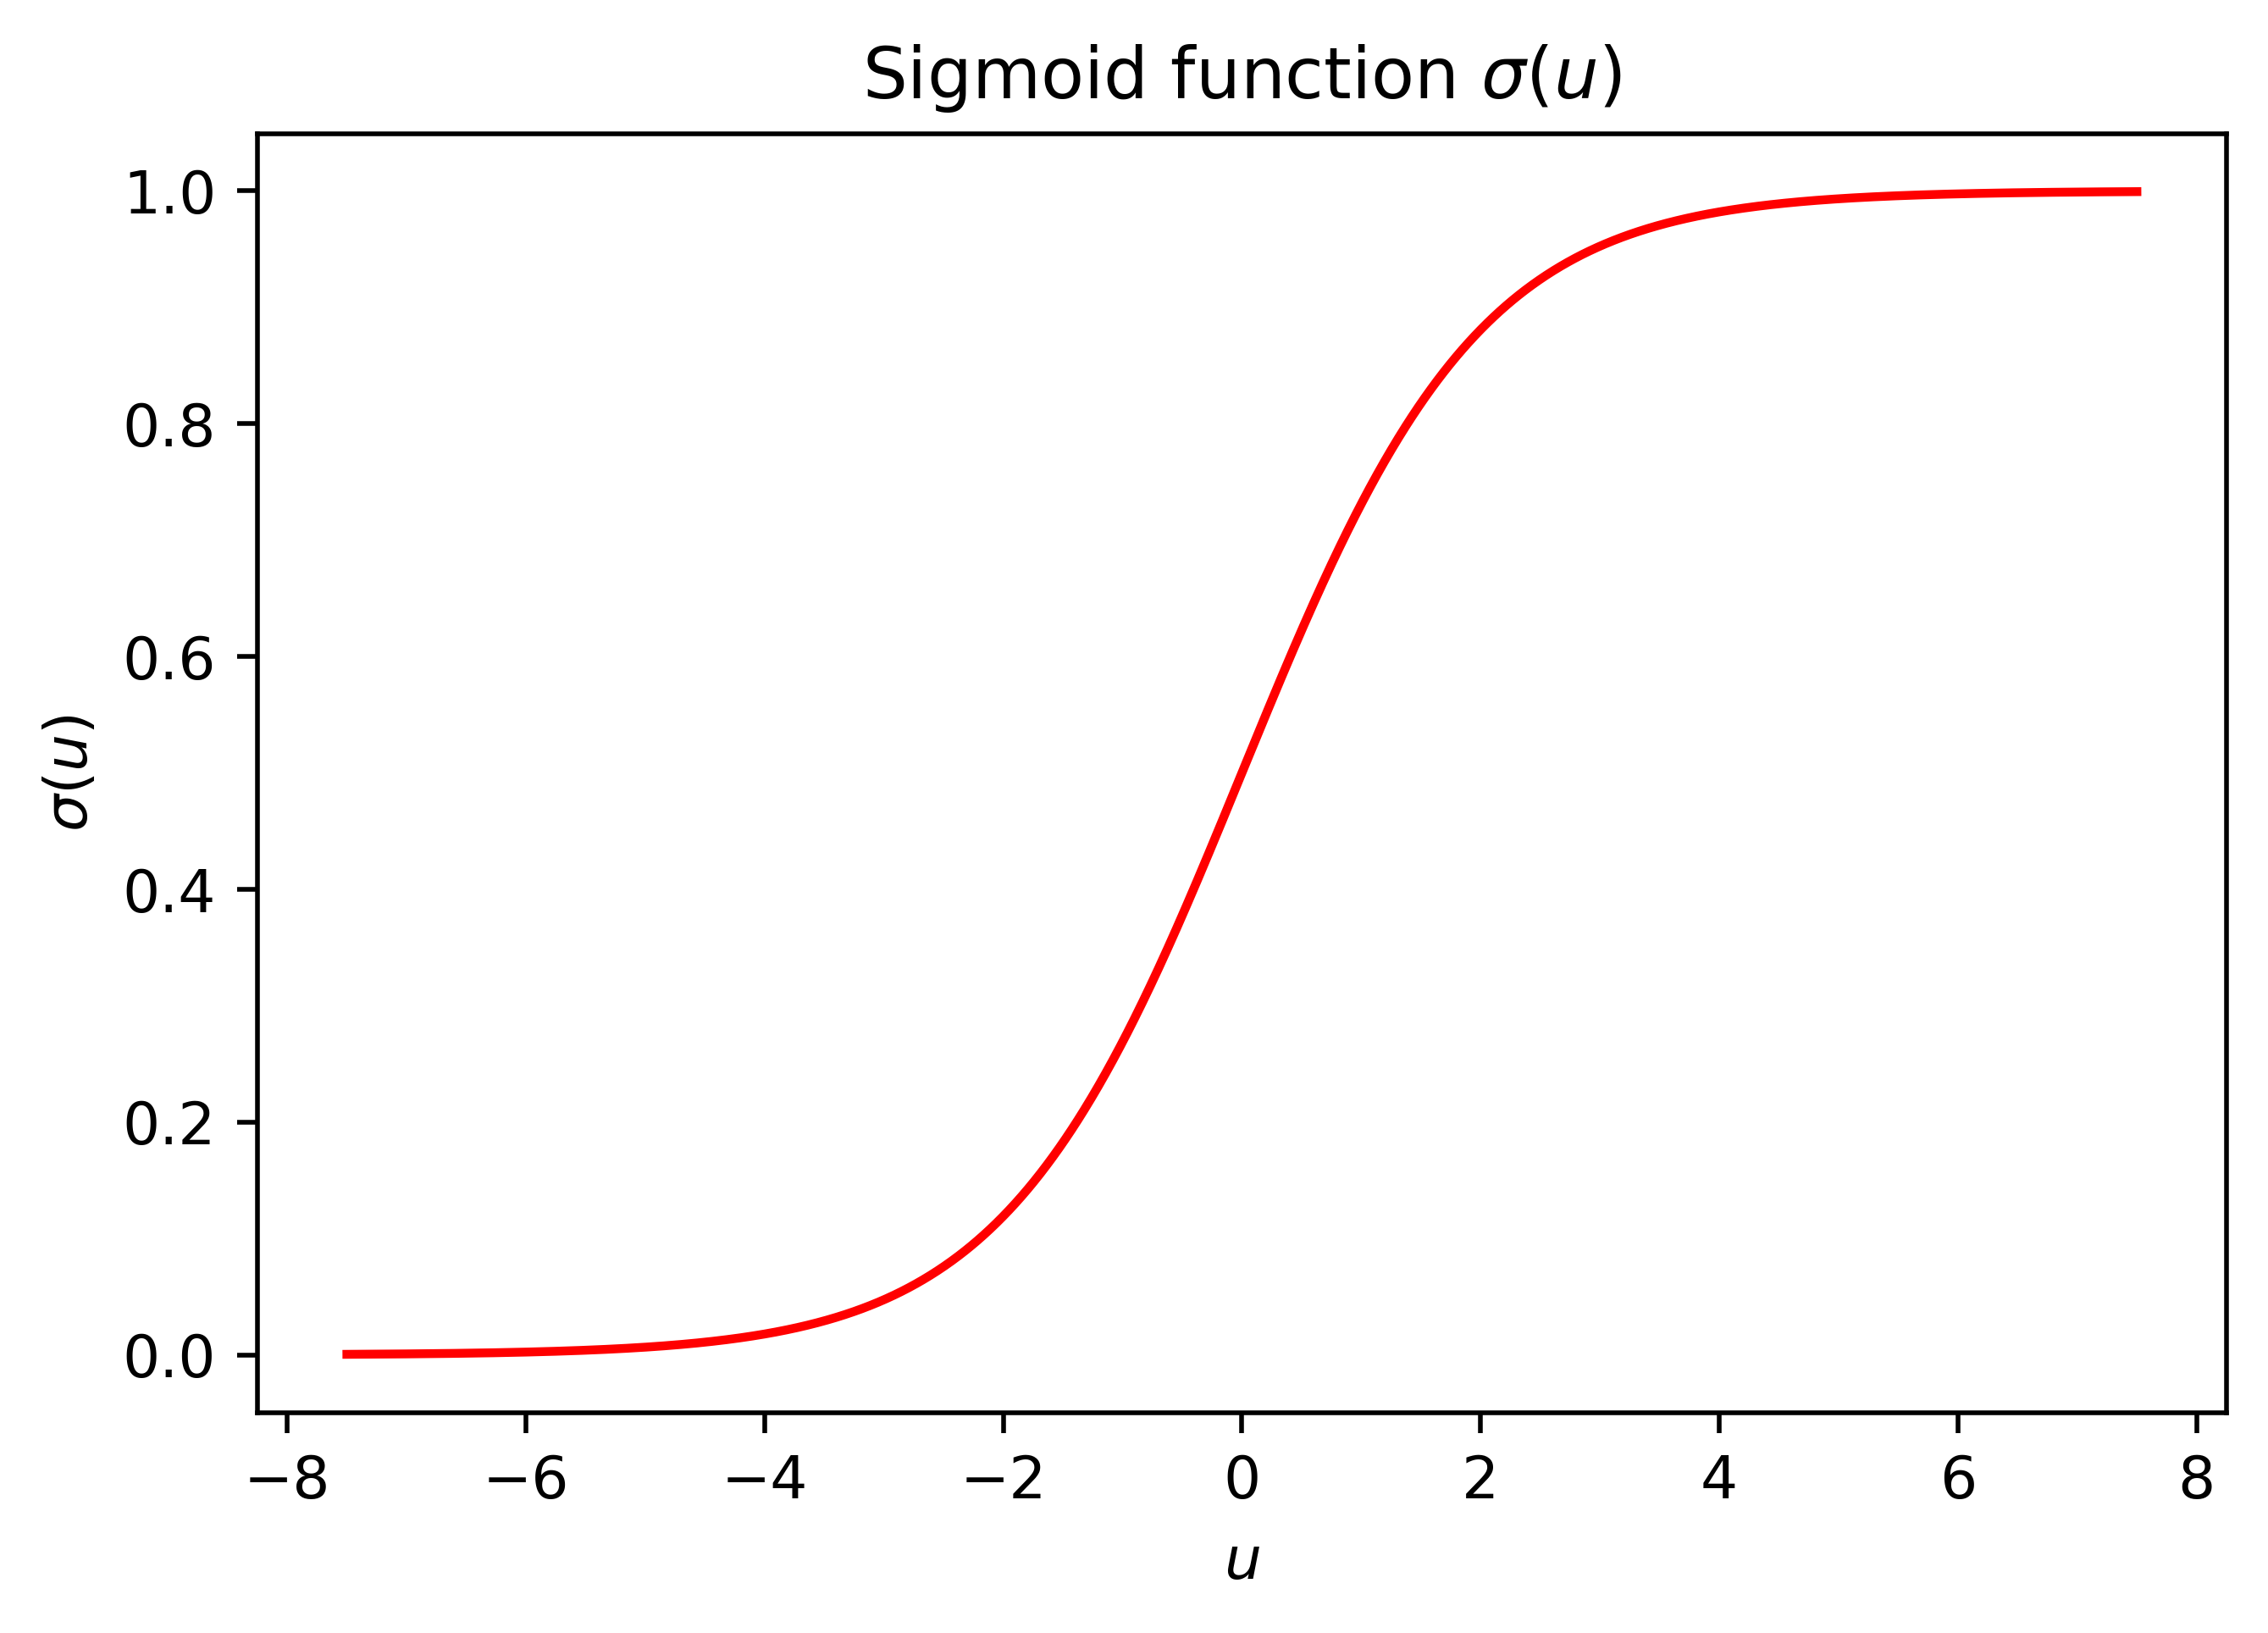
\includegraphics[width=70mm,scale=0.5]{images/feature_images/sigmoid_u.png}
            \caption*{Your friendly neighborhood sigmoid.}
        \end{figure}
    
        Can we use this to create a new model class? For now, unfortunately not: remember that we used this in the last chapter, and we still got a \textbf{linear} separator. The reasons were discussed there.
            \note{We'll show ways we can use this kind of approach, when we discuss Neural Networks.}
    
        Instead, we can get inspiration from our example of "structural error". For now, let's focus on \textbf{regression} (though classification isn't too different):
    
        \begin{figure}[H]
            
            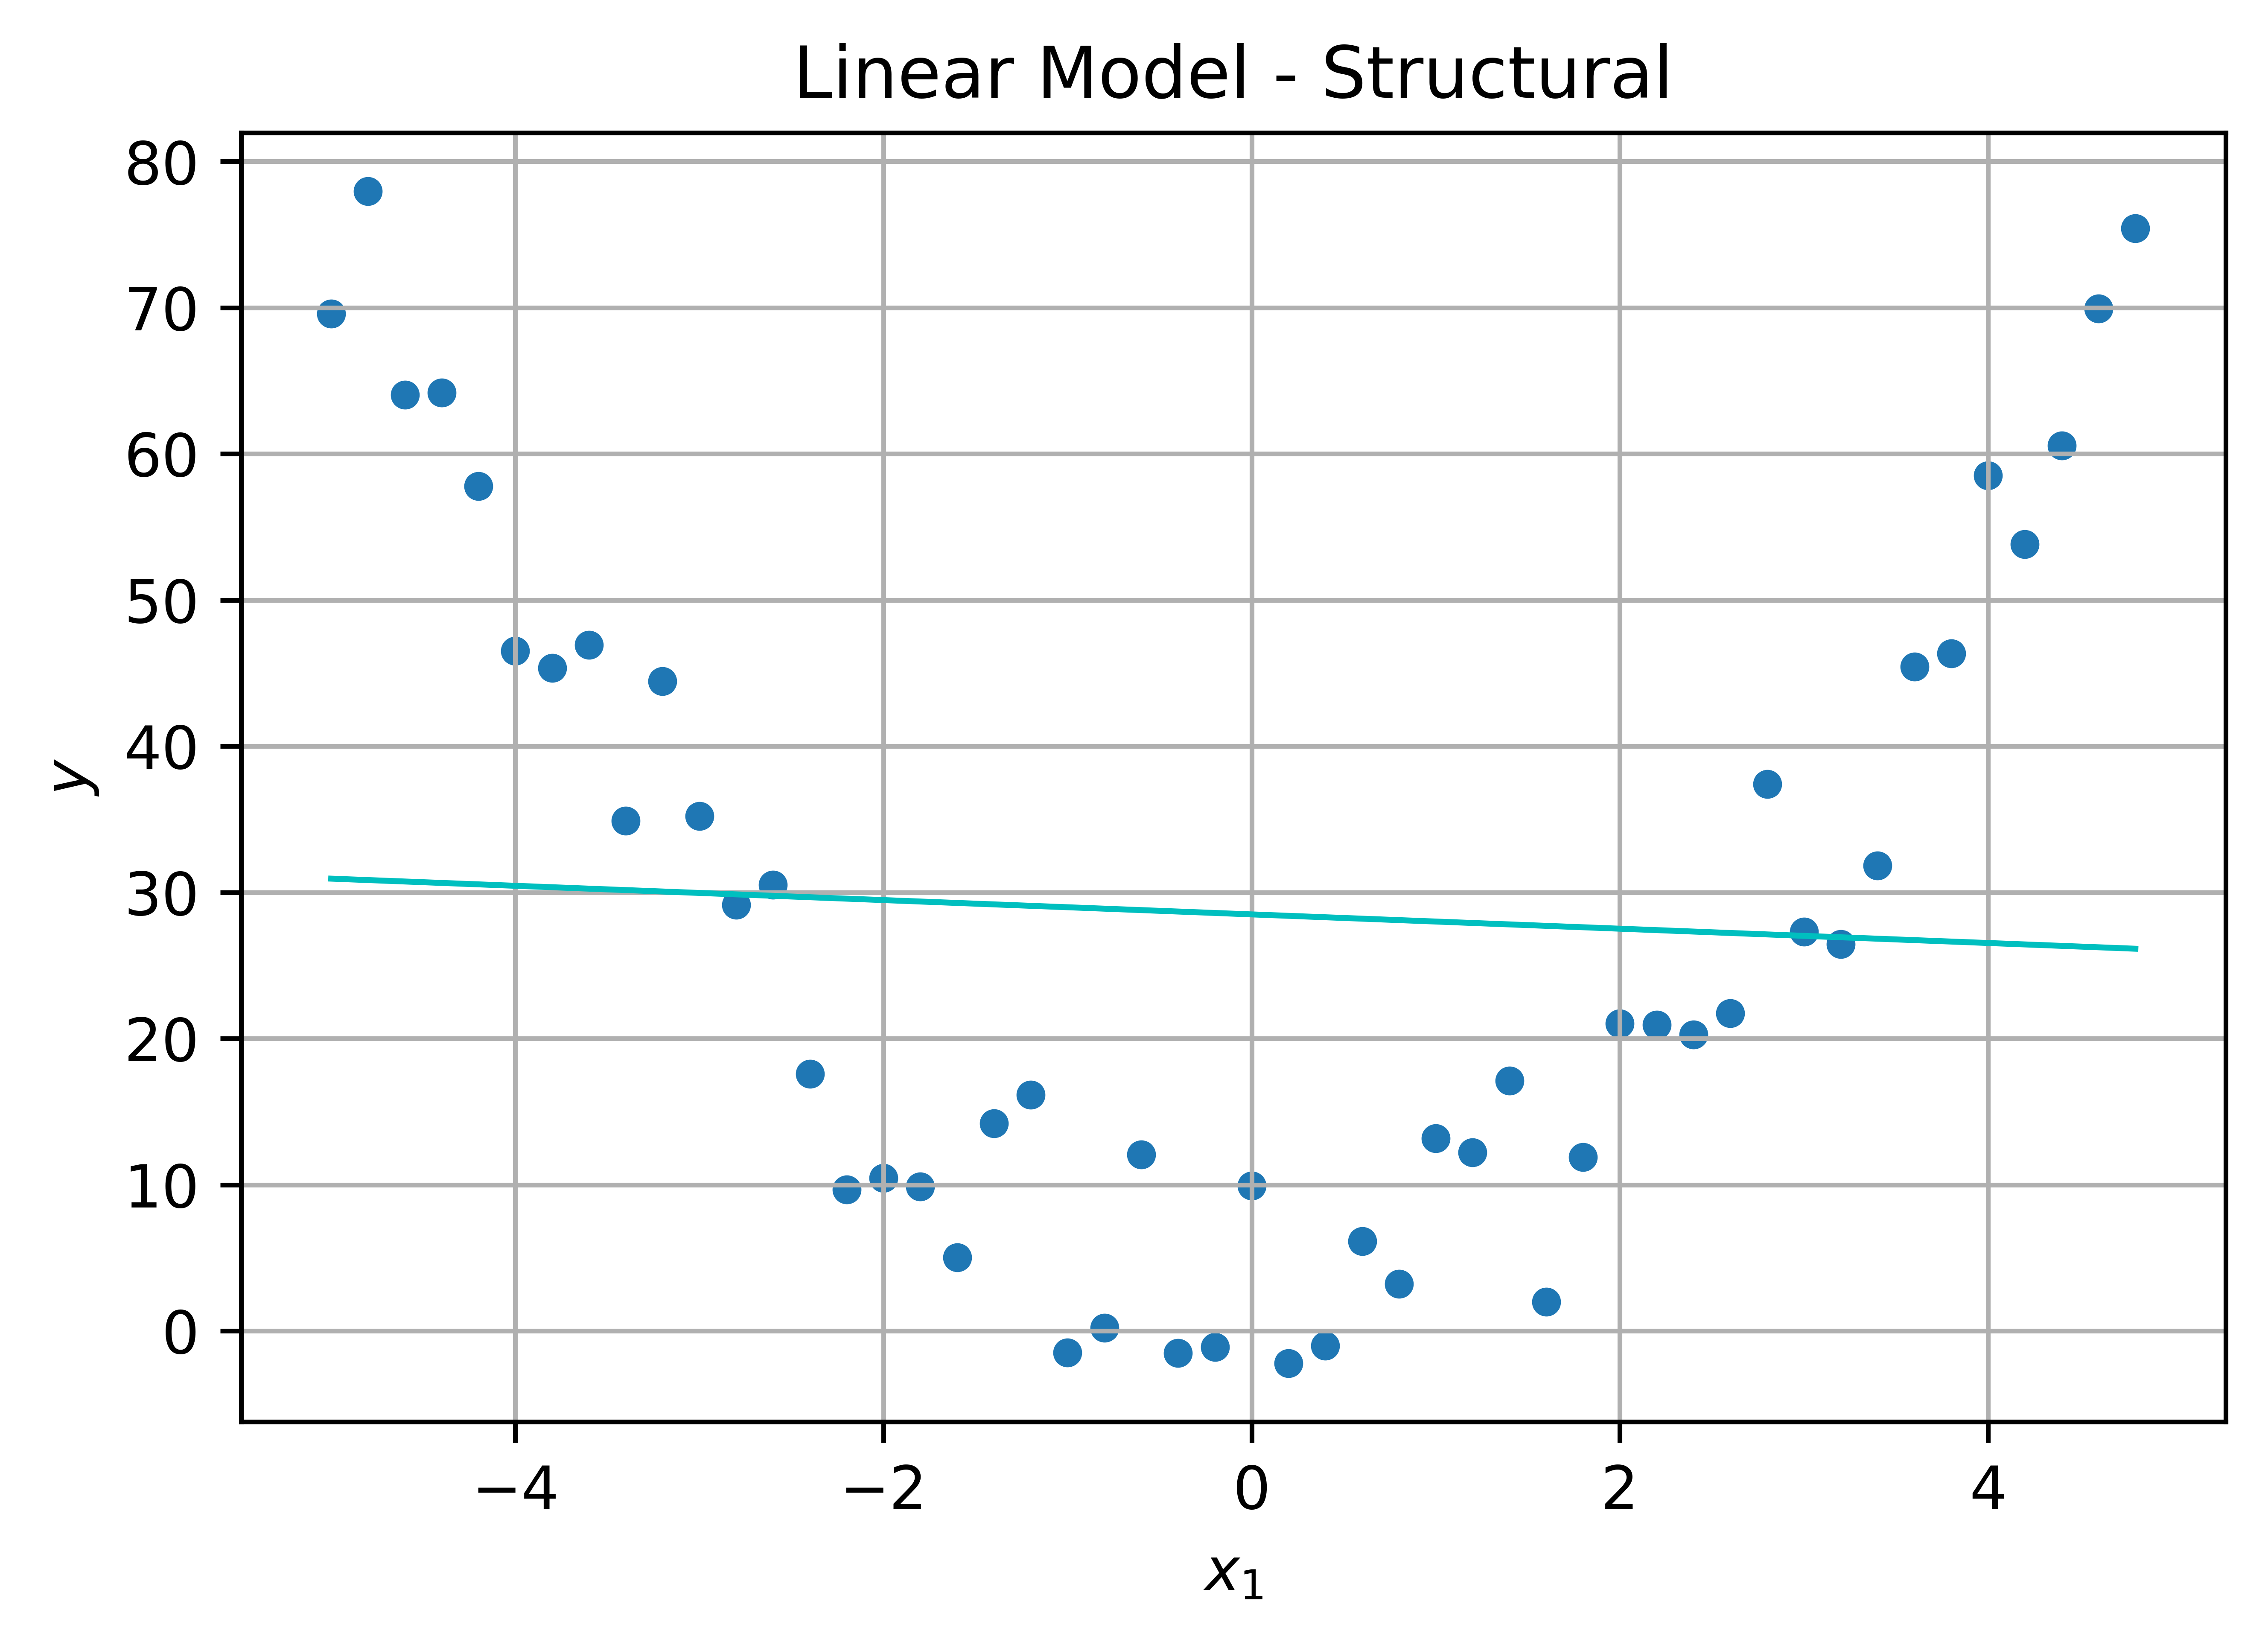
\includegraphics[width=70mm,scale=0.5]{images/feature_images/Structural_Linear_Model.png}
            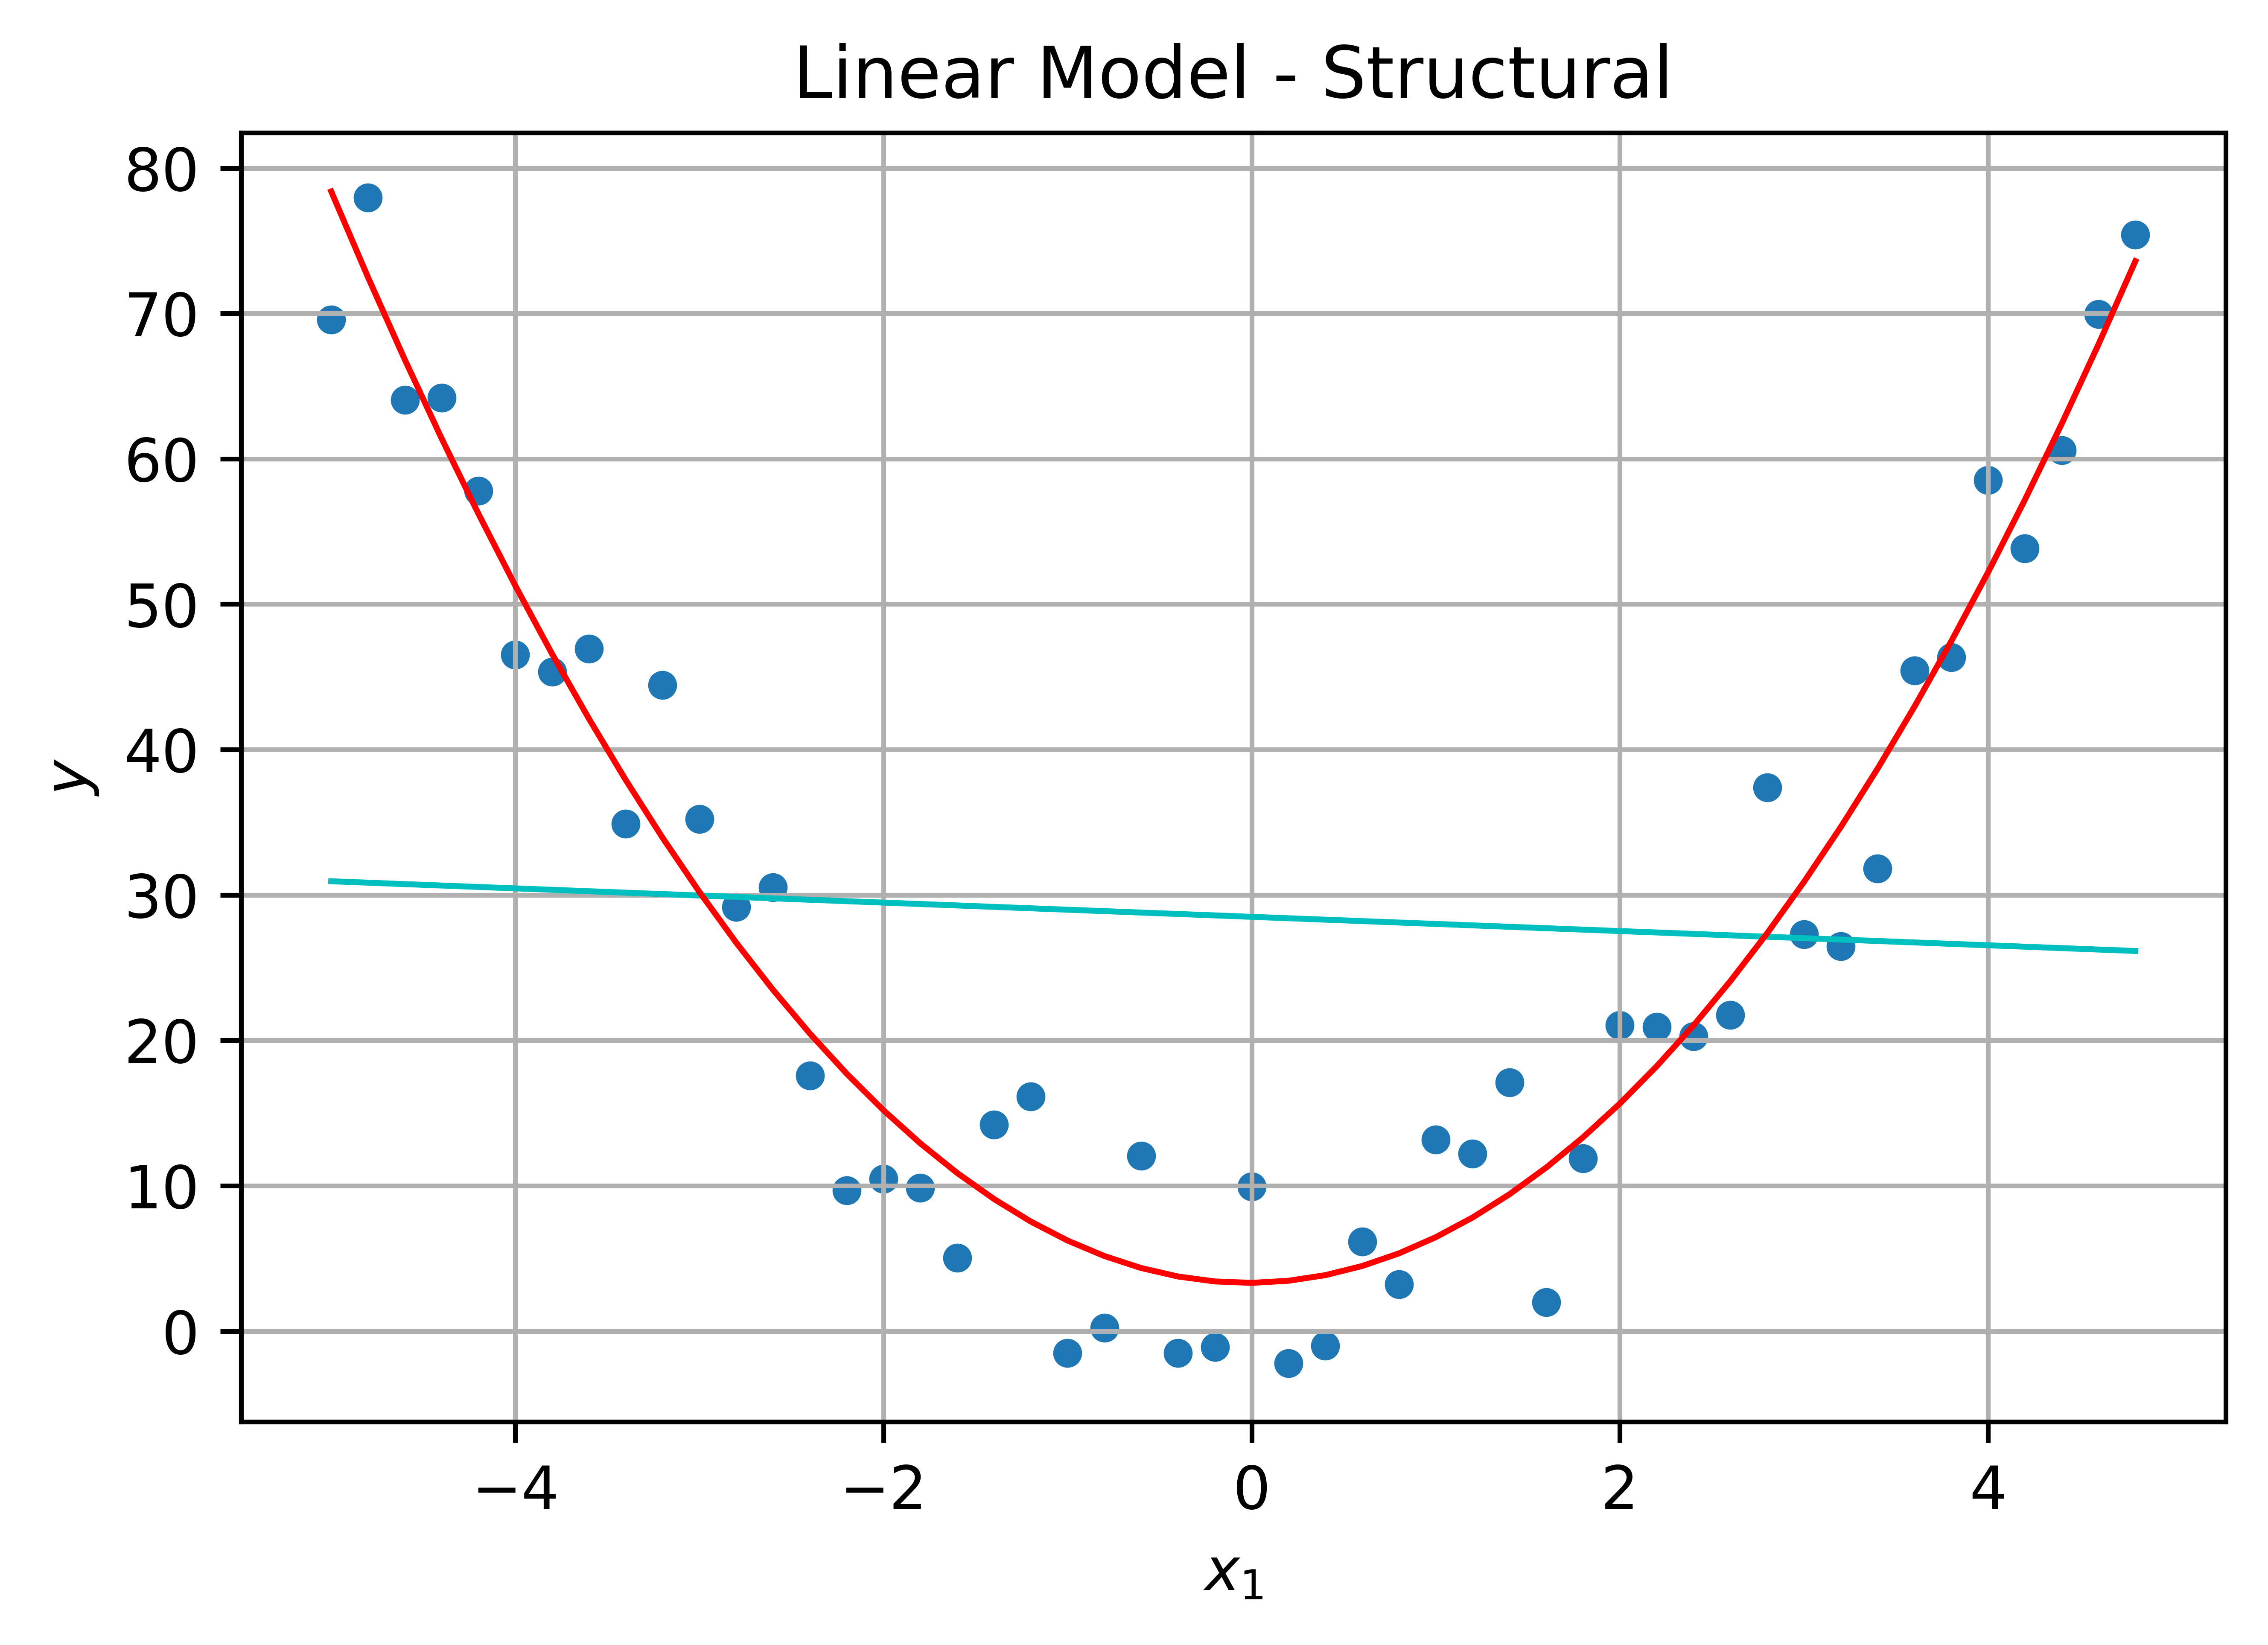
\includegraphics[width=70mm,scale=0.5]{images/feature_images/Structural_Quad_Model.png}
    
            \caption{A linear function can't represent this dataset. However, a parabola can!}
        \end{figure}
    
        We're still using our input variable $x$, but this time, we've "\textbf{transformed}" it: we have squared $x$, giving us a model of the form
            \note{Remember that $x$ is 1-D right now!}
    
        \begin{equation}
            h(x) = \red{A}x^2+\red{B}x+\red{C}
        \end{equation}
    
        It should be clear that his model is more \textbf{expressive} than the one before: it can create every model that our linear approach could (just by setting $A=0$), and it can create new models in a parabola shape.
            \note{Reminder: "expressiveness" or "richness" of a hypothesis class is how many models it can represent: a more expressive model can handle more different situations.}\\
    
        \begin{concept}
            We can make our \purp{linear} model more \gren{expressive} by add a squared term, and turning it into a \purp{parabolic} function.
    
            This concept can be extended even further, to any \vocab{polynomial}.
        \end{concept}

    \subsecdiv
    
    \subsection*{Transformation}
    
        How do we \textit{generalize} this concept? Well, we have a set of constant parameters $A, B, C$. These are similar to our constants $\theta_i$. Let's change our notation:
    
        \begin{equation}
            h(x) = \red{\theta_2} x^2 + \red{\theta_1} x + \red{\theta_0}
        \end{equation}
    
        Now, we've got something more familiar. We could imagine extending this to any number of terms $\theta_i x^i$: if we needed a cubic function, for example, we could include $\theta_3 x^3$.

        This is starting to look pretty similar to our previous model: in fact, we could even separate out $\theta$ as a variable:
            \note{Notice that $\theta_0$ corresponds to $x^0=1$.}

        \begin{equation}
            h(x) = 
            \overbrace{
                \sum_{i=1}^{k}
                \theta_i x^i
            }^{\text{Polynomial sum}}
            =
            \overbrace{
            \begin{bmatrix}
             \theta_0 \\ \theta_1 \\ \theta_2 \\ \vdots \\ \theta_k
            \end{bmatrix}
            \cdot 
            \begin{bmatrix}
                1 \\ x \\ x^2 \\ \vdots \\ x^k
            \end{bmatrix}
            }^{\text{Store as vectors}}
            = 
            \overbrace{
            \theta^T
            }^{\text{Simplify}}
            \begin{bmatrix}
                1 \\ x \\ x^2 \\ \vdots \\ x^k
            \end{bmatrix}
        \end{equation}

        This really \textit{is} starting to look like our linear transformation! That's helpful: we might be able to use the techniques we developed before.

        In fact, we can argue that they're \textbf{equivalent}: we've just changed what our input vector is. Consider our new input $\phi(x)$:

        \begin{equation}
            \blu{\phi(x)}
            = 
            \begin{bmatrix}
                1 \\ x \\ x^2 \\ \vdots \\ x^k
            \end{bmatrix}
            \qquad \qquad
            h(x) = 
            \red{\theta^T} 
            \overbrace{
            \blu{\phi(x)}
            }^{\text{New input}}
        \end{equation}
        
        This is called \textbf{transforming} our input.\\

        \subsection*{Polynomial Basis}

            At the start of this chapter, we introduced the idea of polynomial transformations. If a linear function isn't "expressive" enough to solve a problem, then we can create a more complex model, based on how many $x^i$ we include. This can be written as:

            \begin{equation}
                h(x) =
                \sum_{i=1}^{k}
                \theta_i x^i
                =
                \begin{bmatrix}
                 \theta_0 \\ \theta_1 \\ \theta_2 \\ \vdots \\ \theta_k
                \end{bmatrix}
                \cdot 
                \begin{bmatrix}
                    1 \\ x \\ x^2 \\ \vdots \\ x^k
                \end{bmatrix}
            \end{equation}

            Another word for this might be a "polynomial \textbf{basis}".\\

            \begin{definition}
                A "\vocab{basis}" is the set of basic, \gren{distinct} elements where every \purp{linear} combination creates a unique item in the \purp{space}.
            \end{definition}

            In this case, each term $x^i$ is part of the "basis": we can use any combination $$\sum_i \theta_i x^i$$ to create a unique polynomial. This allows us to cover our "feature space".



            \subsecdiv
            
            \subsubsection*{Order}
            
                An important question to ask is, "how many terms do we include"?

                We categorize our polynomials based on the highest exponent included: this is called the \textbf{order}.\\

                \begin{definition}
                    \vocab{Order} $k$, also known as \vocab{degree}, is the \purp{largest} exponent allowed in our \gren{polynomial}. 

                    Every higher exponential $x^{j}$ can be thought of as having a coefficient $\theta_k=0$: as far as we're concerned, it \gren{doesn't exist}.
                \end{definition}

                \miniex We can compare different orders, by looking at the feature vector they create:
                    \note{Note that, while we chose every coefficient to be nonzero here, they don't have to be! $-x^2+2$ from before is a valid second-order polynomial.}

                Here's a table of the first few:\\

                \begin{center}
                    \begin{tabular}{c c c}
                    Order & $d=1$ & Example \\
                    \hline
                    0 & $[1]$ & $3.5$  \\
                    1 & $[1,x]^T$ & $2.5x-1$ \\
                    2 & $[1,x,x^2]^T$ & $4.1x^2-10x+1$ \\
                    3 & $[1,x,x^2,x^3]^T$ & $x^3+8x^2+x-\sqrt{2}$ \\
                    $\vdots & \vdots & \vdots$
                    \end{tabular}
                \end{center}

                \phantom{}

                The order we choose is an important decision choice.
                
            \subsecdiv

            \subsubsection*{Overfitting with order}
                It's difficult to know how many terms to include in our polynomial, but we run into two problems if our order is \textbf{too high}:

                \begin{itemize}
                    \item It becomes time-consuming to calculate, with little benefit
                    \item We start overfitting more and more.
                \end{itemize}

                The first part makes sense: with more terms, we have to do more multiplications, more additions, etc.\\
                
                \begin{concept}
                    More \vocab{complex models} tend to be more \purp{expensive} to train, and slower to use. This is a trade-off for more \gren{accuracy}. 
                    
                    Usually, there's a point where cost \gren{outweights} benefits. A problem is rarely perfectly solved, even by an excellent model, so you can't just continue until it's "perfect".
                \end{concept}

                But what about the second part? Why do we increase overfitting? 

                With a higher order, our polynomial becomes more complex: it can take on more shapes, which are increasingly complex and perfectly fit to the data.

                This can cause our data to overlook obvious patterns, and instead create a very precise shape that is paying attention to the noise in our model.\\

                \begin{concept}
                    \vocab{High-order polynomials} are very vulnerable to \purp{overfitting}.

                    Because they can take on so many different, \gren{complex} functions, they can very very closely \purp{match} the original data set. 
                    
                    This can cause the model to "learn" noise, and \gren{miss} broader and simpler patterns that actually exist. In may fail to learn something broad and useful, while \purp{memorizing} the dataset with its expressiveness.
                \end{concept}

                Let's see this in action: we'll generate some data based on $2x+1$, while applying some random noise to it. We'll see the optimized linear regression model for each.
                    \note{For ease, we'll exclude regularization: it does help mitigate this problem, but it doesn't totally solve it.}

                Rather than transform the data, we'll transform the separator: this really highlights the overfitting effect.

                \begin{figure}[H]
                    \centering
                    
                    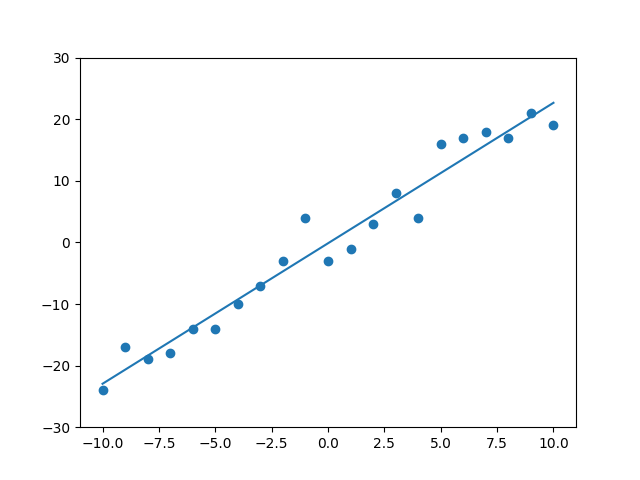
\includegraphics[width=70mm,scale=0.5]{images/feature_images/order_1_soln.png}
                    \caption*{Here's the 1st order solution: in this case, correct for the underlying distribution. It fits our data fine.}
                \end{figure}

                \begin{figure}[H]
                    \centering
                    
                    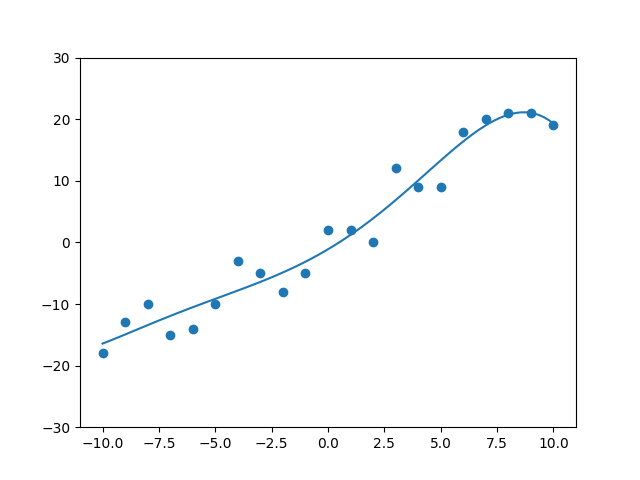
\includegraphics[width=60mm,scale=0.5]{images/feature_images/order_5_soln.png}
                    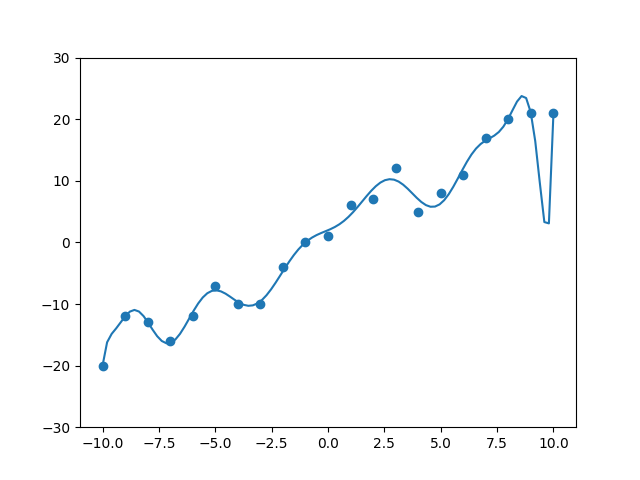
\includegraphics[width=60mm,scale=0.5]{images/feature_images/order_15_soln.png}
                    \caption*{5th and 15th order. The left model looks suspicious, and the right is way overfit. It's very unlikely that we know such an intricate pattern, from so little data.}
                \end{figure}

                 \begin{figure}[H]
                    \centering
                    
                    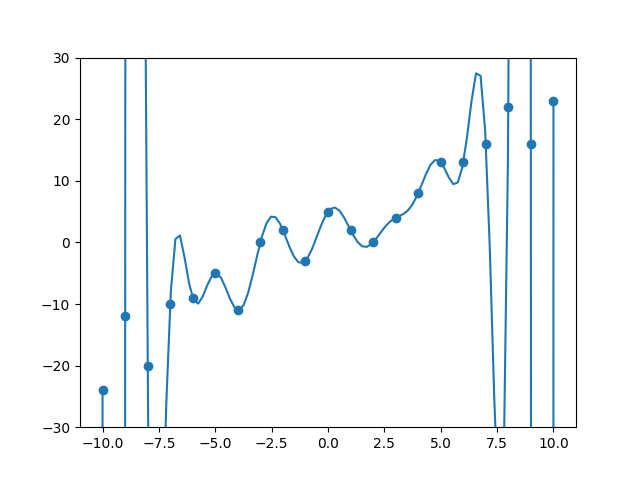
\includegraphics[width=70mm,scale=0.5]{images/feature_images/order_20_soln.png}
                    \caption*{20th order. We have one order for each data point: now, our model is capable of doing regression going through every single data point: as overfit as physically possible, perfectly matching the data.}
                \end{figure}

            \subsecdiv
            \subsubsection*{Higher dimensions}

                Until now, we've only been focusing on the 1-D case of data. Let's change that. Let's consider a 2D dataset $[x_1,x_2]^T$.

                Our typical model

                \begin{equation}
                    \theta^Tx + \theta_0 = \theta_1x_1 + \theta_2x_2 + \theta_0
                \end{equation}

                Is "order 1": the largest exponent is 1. This is still a "linear" model. 

                If we want to move up to order 2, we increase the max exponent, adding $x_1^2$ and $x_2^2$ to the basis.

                However, this doesn't take full advantage of the expressiveness of our model: this only creates parabolas aligned with the $x_1$ and $x_2$ axes. How do we create other options?

                Well, we created these options by multiplying $x_1$ with another $x_1$. It seems like we could logically expand to multiplying $x_1$ by $x_2$.\\

                \begin{definition}
                    For \vocab{higher dimension} $d>1$ \vocab{polynomials}, we allow for multiplication \purp{between variables} $x_i$ and $x_j$.

                    The \vocab{order} of the polynomial is the maximum number of times you can \purp{multiply variables} together. 
                    
                    For order $k$, the \gren{sum of exponents} must be \purp{less than or equal to} the order.
                \end{definition}

                So, for $d=2$, order=$2$, we get the basis:

                \begin{equation}
                    \begin{bmatrix}
                        1 & x_1 & x_1^2 & x_2 & x_2x_1 & x_2^2
                    \end{bmatrix}^T
                \end{equation}

                For $d=2$, order=$3$, it starts getting a bit messy: we have 10 different basis terms.
                    \note{You don't need to memorize these.}

                \begin{equation}
                    \begin{bmatrix}
                        1 & x_1 & x_1^2 & x_1^3 &
                        x_2 & x_2x_1 & x_2x_1^2 & x_2^2 &
                        x^2x_1 & x^3
                    \end{bmatrix}^T
                \end{equation}

            \subsecdiv
            \subsubsection*{Total number of features}
        
                How many do we have in general? Well, every term results from multiplying variables \textbf{at most} $k$ times. Or, the exponents \textbf{add up} to at most $k$.
                
                If we count 1 as a factor, we can say that the exponents always add up to $k$ (since $1^j$ has no effect). So, we have $d+1$ different numbers, which add up to exactly $k$.
                    \note{We have $d$ variables, so $d+1$ if we include 1 as a variable.}

                This is a well-known problem in combinatorics: how many ways are there to add up $m$ numbers to total $n$? The solution to this problem gives us:
                    \note{Explaining the math here is beside the point of this course. If you're curious, search up "stars and bars math", or visit \href{https://en.wikipedia.org/wiki/Stars_and_bars_(combinatorics)}{here}.}

                \begin{equation}
                    \binom{(d+1)+k-1}{k} = \binom{d+k}{k} = \frac{(d+k)!}{d!k!}
                \end{equation}

            \subsecdiv
            \subsubsection*{Summary of Polynomial Basis}

                \phantom{}

                \begin{definition}
                    The \vocab{polynomial basis} of order $k$ and dimension $d$ includes \purp{every feature}

                    \begin{equation}
                        \prod_{i=1}^d x_i^{c_i}
                    \end{equation}

                    Where all of the integer exponents $c_i\geq 0$ add up to \gren{at most} $k$.

                    Creating features such as:

                    \begin{equation}
                        x_1^k, \;\; x_1x_2, \;\; x_2x_3^3x_6, \;\; 1, \;\; \dots
                    \end{equation}
                \end{definition}

                We can represent this in a table:
                    \note{This table is different from the one we saw earlier!}

                \begin{center}
                    \begin{tabular}{c c c}
                    Order & $d=1$ & in general ($d>1$) \\
                    \hline
                    0 & $[1]$ & \red{$[1]$}\\
                    1 & $[1,x]^T$ & \red{$[1,x_1, \ldots, x_d]^T$}\\
                    2 & $[1,x,x^2]^T$ & \red{$[1,x_1, \ldots, x_d,
                                        x_1^2, x_1x_2, \ldots]^T$}\\
                    3 & $[1,x,x^2,x^3]^T$ & \red{$[1,x_1, \ldots,
                                        x_1^3, x_1x_2, \ldots,
                                        x_1x_2x_3, \ldots]^T$} \\
                    $\vdots$ & $\vdots$ & $\vdots$ \\
                    \end{tabular}
                \end{center}

            \subsecdiv

        \subsubsection*{Polynomial Basis in Action}

            Below, we'll show examples of how polynomial basis being used, to demonstrate just how useful it is.

            But how do we use feature transformations? The best part: remember that we can view it as a linear separator? We can train it just the same way!\\

            \begin{concept}
                \vocab{Feature transformations} \purp{don't change} how we train our model. We can still treat our model as a \gren{linear} vector $\theta$, even if our data has been \gren{non-linearly} transformed. 

                So, after we transform our data, we can use normal techniques (OLS, gradient descent, SGD) to fit our model.
            \end{concept}

            In this situation, the benefits of regularization become more clear: by preventing $\theta$ from becoming too large, we discourage a surface that is too "extreme", with larger changes across its surface.

            We'll train our model for various situations, to see what it can do. Different problems require different orders $k$, still.
            
            \begin{figure}[H]
                \centering
                
                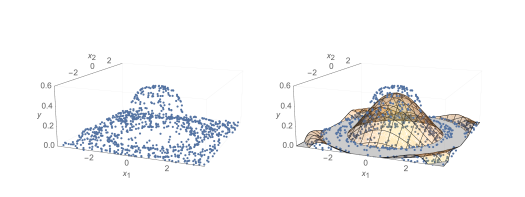
\includegraphics[width=80mm,scale=0.5]{images/feature_images/vibrations.png}
                \caption*{We start with the waveform we showed at the start of the chapter: on the left, we see a bunch of datapoints we want to take a regression over. With $k=8$, we get a pretty good result.}
            \end{figure}

            \begin{figure}[H]
                \centering
                
                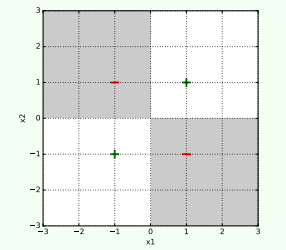
\includegraphics[width=70mm,scale=0.5]{images/feature_images/xor.png}
                \caption*{This is the classic "xor" problem: a typical case of "linearly unseparable". With $k=2$, we can classify it well with the chosen model $4x_1x_2=0$.}
            \end{figure}

            \begin{figure}[H]
                \centering
                
                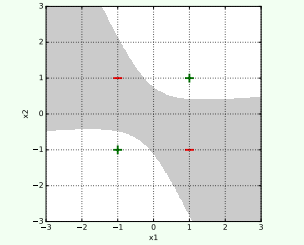
\includegraphics[width=70mm,scale=0.5]{images/feature_images/better_xor.png}
                \caption*{This time we use gradient descent and a random initialization to get a less 'perfect', but still effective classification. }
            \end{figure}

             \begin{figure}[H]
                \centering
                
                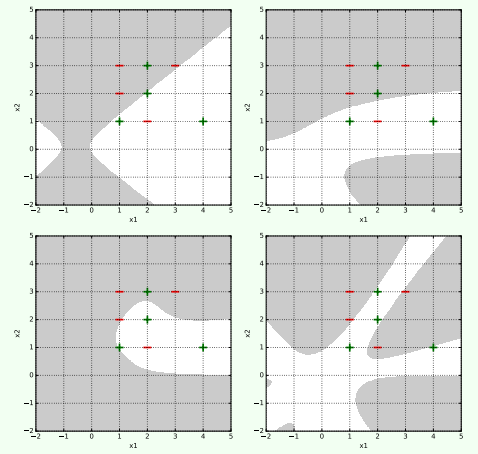
\includegraphics[width=70mm,scale=0.5]{images/feature_images/harder_dataset.png}
                \caption*{This dataset is pretty brutal: we try with $k=2,3,4,$ and finally $5$. The shapes we get are... complex, to say the least. But, we successfully solve it with $k=5$.}
            \end{figure}
